\section{Introduction}

After discovering Higgs boson\cite{20121, 201230}, the examine of electroweak symmetry breaking (EWSB) becomes a main focus at the LHC.
In addition to measuring the properties of Higgs boson directly, the vector boson scattering (VBS) process is another key avenue to probe EWSB\cite{Lee:1977yc, Chanowitz:1985hj, Szleper:2014xxa}.
As introduced in section~\ref{symbreaking}, in Standard Model (SM), the Higgs boson acts as "moderator" to unitarize high-energy longitudinal VBS amplitudes at the TeV scale.
Therefore, studying high-energy behaviours of VBS is crucial to understand the mechanism of EWSB.

Since no VBS process was observed prior to the LHC era, LHC provides an unexceptionable opportunity to study them due to its unprecedented high energy and lunimosity.
At LHC, the VBS process is typically studied through the measurements of electroweak (EW) production of two vector bosons radiated from initial-state quarks 
plus a pair hadronic jets with high energy in the back and forward regions (denoted as EW-VVjj).
The quantum chromodynamics (QCD) production of VVjj contains two QCD vertices at the lowest order (denoted as QCD-VVjj) is an inreducible background to the search of EW-VVjj production.
The features of EW-VVjj production include a large invariant mass of jet pair ($m_{jj}$) and a significant separation of rapidity between two jets ($\Delta y_{jj}$).
Figure~\ref{fig:vbszz_diagrams} presents some typical Feynman diagrams of EW- and QCD-ZZjj processes.
\begin{figure}[!htbp]
\begin{center}
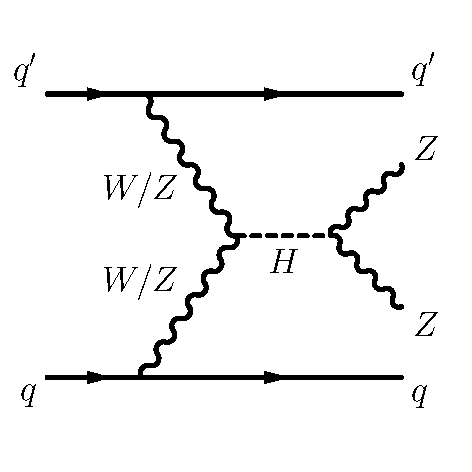
\includegraphics[width=0.22\textwidth]{figures/VBSZZ/diagram-EWZZjj-Schn-Higgs.pdf}
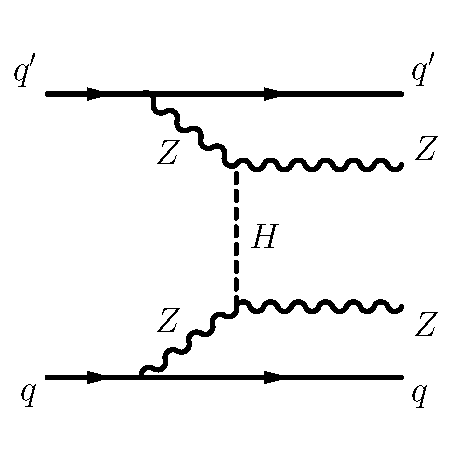
\includegraphics[width=0.22\textwidth]{figures/VBSZZ/diagram-EWZZjj-Tchn-Higgs.pdf}
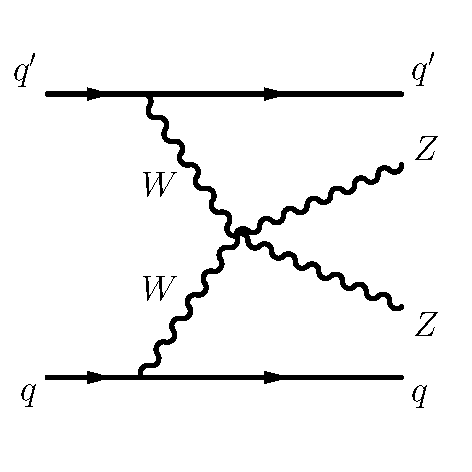
\includegraphics[width=0.22\textwidth]{figures/VBSZZ/diagram-EWZZjj-QGC.pdf}
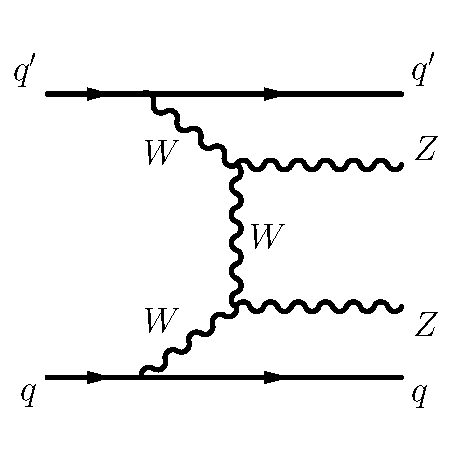
\includegraphics[width=0.22\textwidth]{figures/VBSZZ/diagram-EWZZjj-TGC.pdf}\\
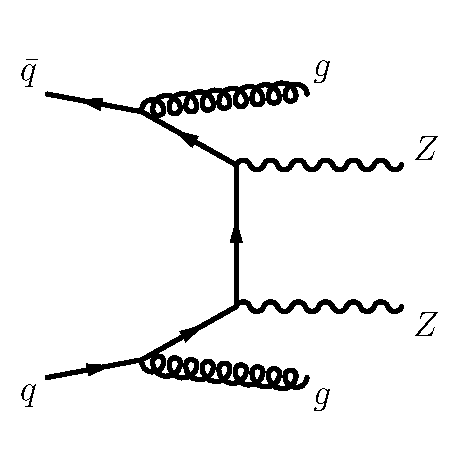
\includegraphics[width=0.22\textwidth]{figures/VBSZZ/diagram-QCDZZjj-qq.pdf}
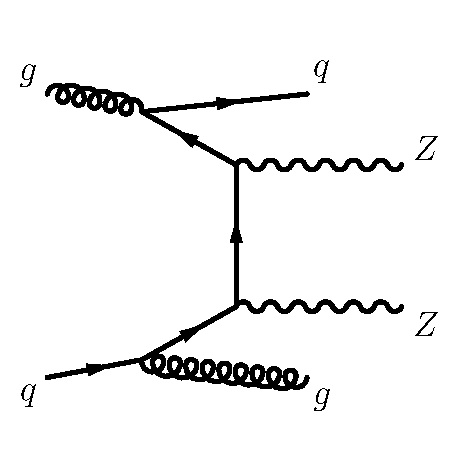
\includegraphics[width=0.22\textwidth]{figures/VBSZZ/diagram-QCDZZjj-qg.pdf}
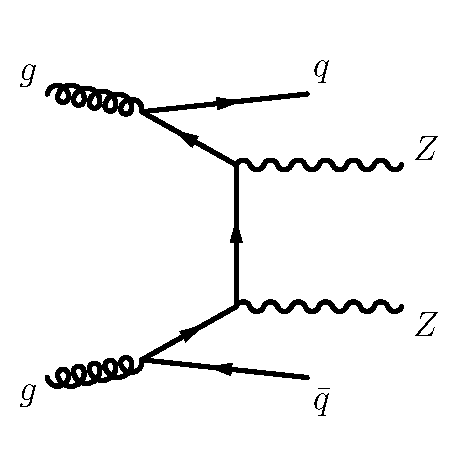
\includegraphics[width=0.22\textwidth]{figures/VBSZZ/diagram-QCDZZjj-gg.pdf}
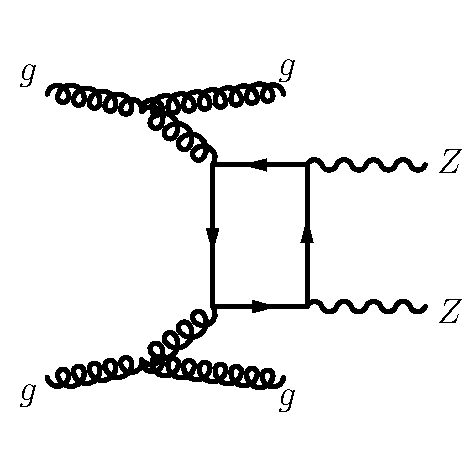
\includegraphics[width=0.22\textwidth]{figures/VBSZZ/diagram-QCDZZjj-box.pdf}\\
\end{center}
\caption{Typical diagrams for the production of $ZZjj$, including the relevant EW VBS diagrams (first row) and QCD diagrams (second row).}
\label{fig:vbszz_diagrams}
\end{figure}

The first evdience of the EW-VVjj process was seen in same-sign WW channel (EW-$W^{\pm}W^{\pm}$jj) by ATLAS collaboration with 20.3~\ifb~8~\tev~data\cite{PhysRevLett.113.141803},
in which a 3.6$\sigma$ excess was observed in data over the background-only prediction.
In LHC run-2, the observation of EW-$W^{\pm}W^{\pm}$jj process has been reported in both ATLAS and CMS collabration with 36~\ifb~13~\tev~data\cite{PhysRevLett.123.161801, Sirunyan:2017ret}.
In WZ channel (EW-WZjj), an observation with 5.3$\sigma$ excess was also reported by the ATLAS collabration recently\cite{2019469}.
The EW production in ZZ final state (EW-ZZjj) is typically rare, whose fiducial cross section has an order of \textit{O}(0.1)~\ifb in the final state where both Z bosons decay leptonically.
The EW-ZZjj production was searched by CMS using 35.9~\ifb~13~\tev~data, no evidence was found\cite{2017682}.
But in the meantime, $ZZ \rightarrow 4l$ process offers a extramely clean channel than all the others, with more data collected in LHC, the observation of EW-ZZjj becames possible.

This section will present the first observation of EW-ZZjj production by ATLAS collabration using the complete set of LHC run-2 data with 139~\ifb luminosity.
It is a new milestone in the study of EWSB at LHC, and completes the last missing part of observation of weak boson scattering for \textit{massive bosons}.
The thesis will focus on the final state of Z bosons pair decay to four charged leptons with two jets (\llll jj), includes both search of EW production and the fiducial cross-sections measurement for the inclusive production of the EW and QCD processes.
The ZZjj production involving intermediate $\tau$-leptons from Z decays is considered as signal but has a negligible contribution to the selected event sample.
Reducible backgrounds give minor contributions in the \llll jj channel.
To further separate the EW signal and the QCD background, multivariate discriminant (MD) is trained using event kinematic information from simulated samples. 
The MD distribution is then used as discriminant in statistical fit to evaluate the signal strength of EW process.
